\documentclass{standalone}
\usepackage{tikz}
\usetikzlibrary{patterns, positioning}
\usepackage[sfdefault]{ClearSans} %% option 'sfdefault' activates Clear Sans as the default text font
\usepackage[T1]{fontenc}

\begin{document}
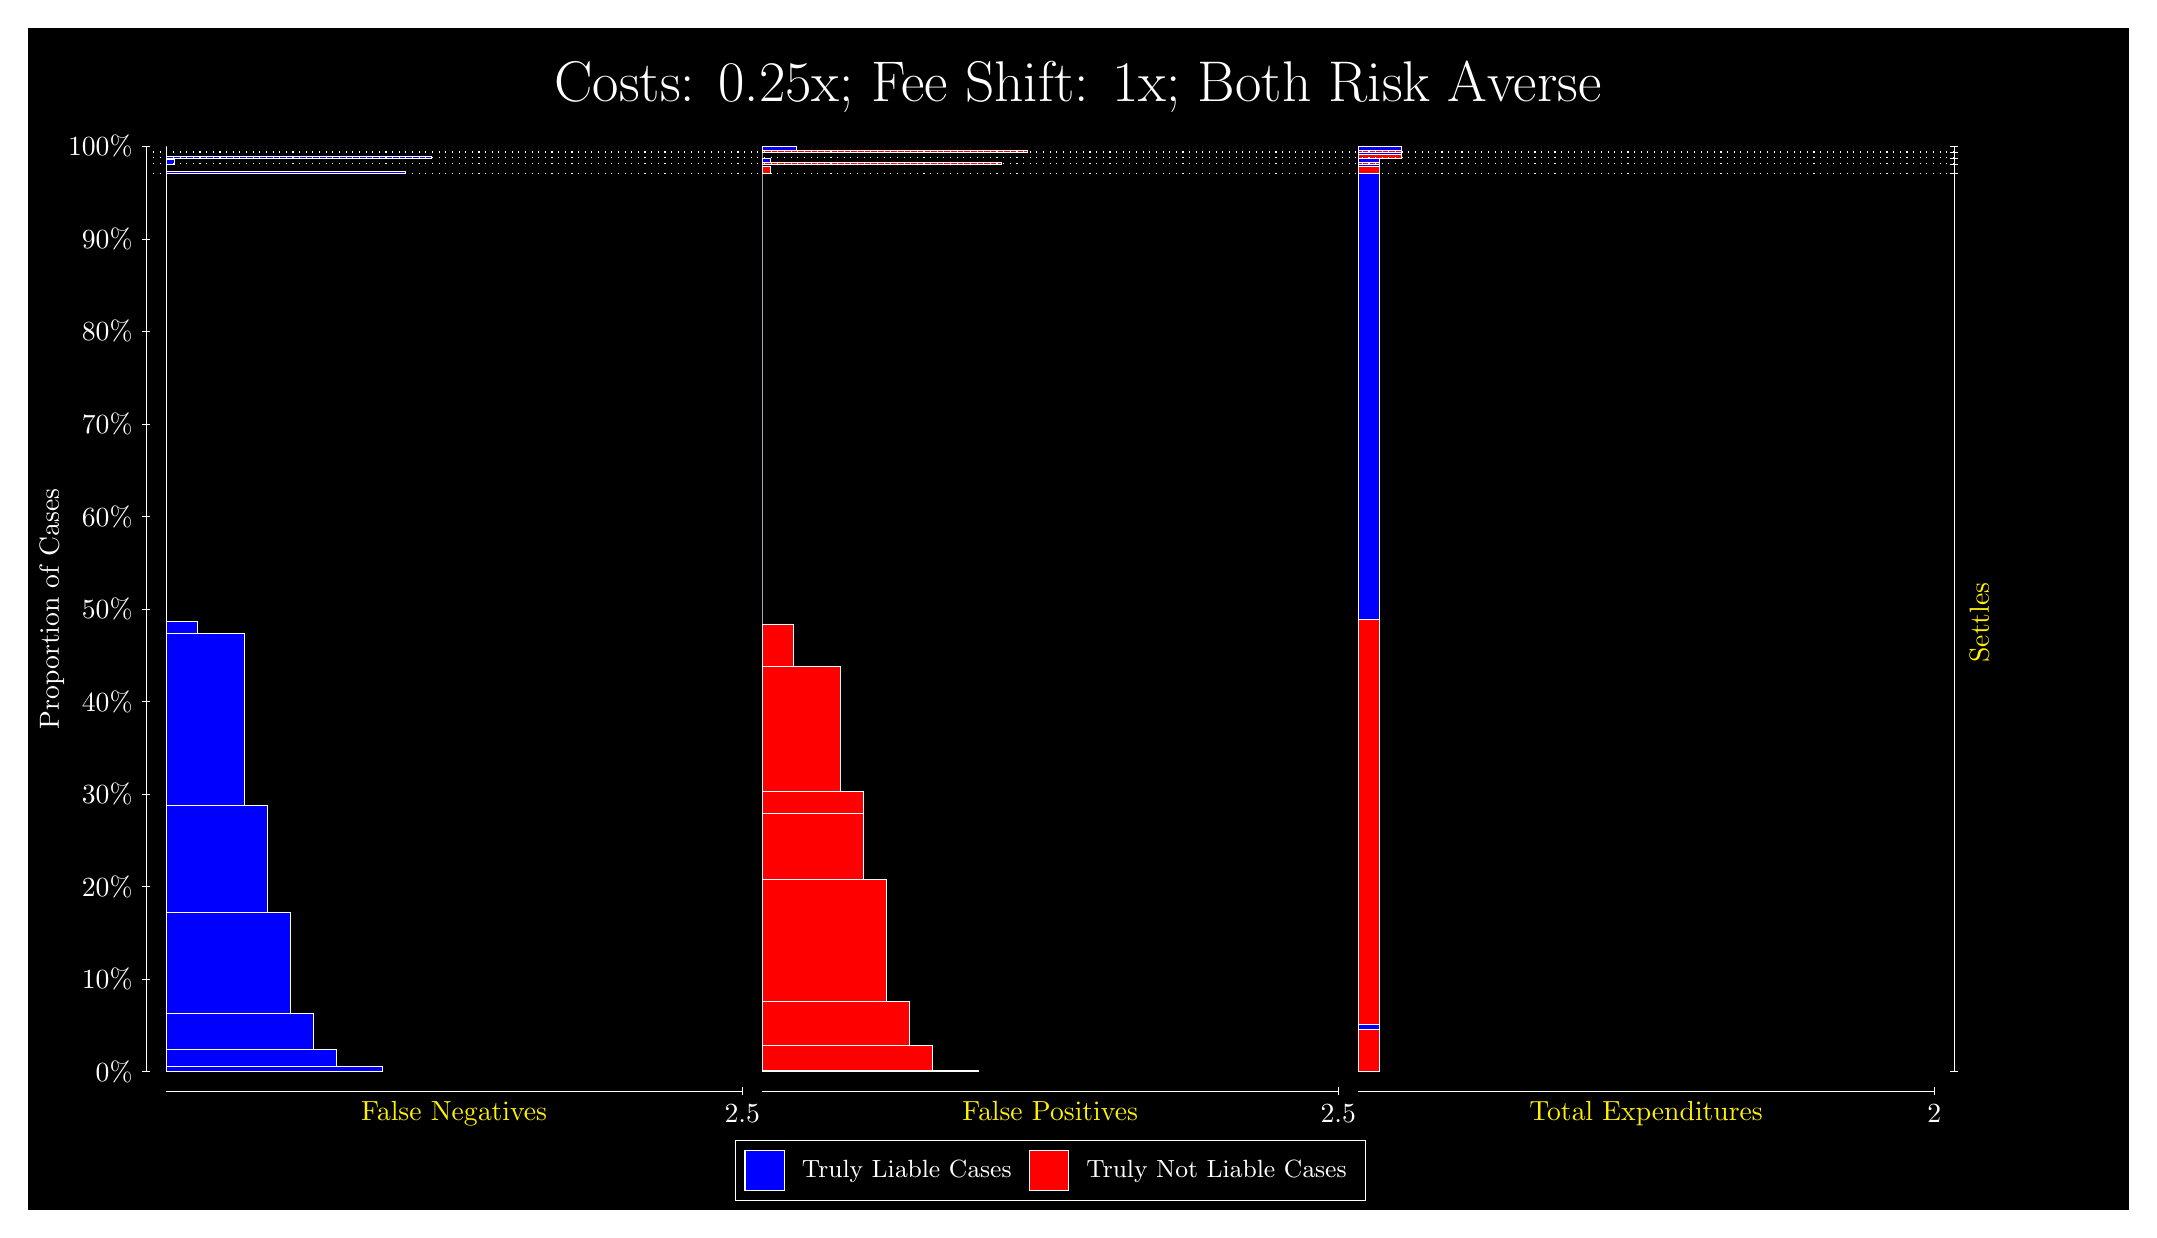
\begin{tikzpicture}
\draw[fill=black] (0,0) rectangle (26.667,15);
\draw[text=white] (0,13.5) rectangle (26.667,15) node[midway] {\huge Costs: 0.25x; Fee Shift: 1x; Both Risk Averse};
\draw[white, very thin] (1.5,1.75) -- (1.5,13.5);
\node[rotate=90, text=white, anchor=center] at (0.3, 7.625) {Proportion of Cases};
\draw[white, very thin] (1.45,1.75) -- (1.55,1.75);
\node[text=white, anchor=east] at (1.45, 1.75) {0\%};
\draw[white, very thin] (1.45,2.925) -- (1.55,2.925);
\node[text=white, anchor=east] at (1.45, 2.925) {10\%};
\draw[white, very thin] (1.45,4.1) -- (1.55,4.1);
\node[text=white, anchor=east] at (1.45, 4.1) {20\%};
\draw[white, very thin] (1.45,5.275) -- (1.55,5.275);
\node[text=white, anchor=east] at (1.45, 5.275) {30\%};
\draw[white, very thin] (1.45,6.45) -- (1.55,6.45);
\node[text=white, anchor=east] at (1.45, 6.45) {40\%};
\draw[white, very thin] (1.45,7.625) -- (1.55,7.625);
\node[text=white, anchor=east] at (1.45, 7.625) {50\%};
\draw[white, very thin] (1.45,8.8) -- (1.55,8.8);
\node[text=white, anchor=east] at (1.45, 8.8) {60\%};
\draw[white, very thin] (1.45,9.975) -- (1.55,9.975);
\node[text=white, anchor=east] at (1.45, 9.975) {70\%};
\draw[white, very thin] (1.45,11.15) -- (1.55,11.15);
\node[text=white, anchor=east] at (1.45, 11.15) {80\%};
\draw[white, very thin] (1.45,12.325) -- (1.55,12.325);
\node[text=white, anchor=east] at (1.45, 12.325) {90\%};
\draw[white, very thin] (1.45,13.5) -- (1.55,13.5);
\node[text=white, anchor=east] at (1.45, 13.5) {100\%};

\draw[white, very thin] (24.457,1.75) -- (24.457,13.5);
\draw[white, very thin] (24.407,1.75) -- (24.507,1.75);
\node[anchor=west] at (24.407, 1.75) {};
\draw[white, very thin] (24.407,13.153) -- (24.507,13.153);
\node[anchor=west] at (24.407, 13.153) {};
\draw[white, very thin] (24.407,13.278) -- (24.507,13.278);
\node[anchor=west] at (24.407, 13.278) {};
\draw[white, very thin] (24.407,13.354) -- (24.507,13.354);
\node[anchor=west] at (24.407, 13.354) {};
\draw[white, very thin] (24.407,13.428) -- (24.507,13.428);
\node[anchor=west] at (24.407, 13.428) {};
\draw[white, very thin] (24.407,13.5) -- (24.507,13.5);
\node[anchor=west] at (24.407, 13.5) {};

\draw[white, very thin, fill=blue] (1.75,1.75) rectangle (4.4946,1.8106);
\draw[white, very thin, fill=blue] (1.75,1.8106) rectangle (3.9091,2.0269);
\draw[white, very thin, fill=blue] (1.75,2.0269) rectangle (3.6163,2.493);
\draw[white, very thin, fill=blue] (1.75,2.493) rectangle (3.3236,3.772);
\draw[white, very thin, fill=blue] (1.75,3.772) rectangle (3.0308,5.1269);
\draw[white, very thin, fill=blue] (1.75,5.1269) rectangle (2.738,7.317);
\draw[white, very thin, fill=blue] (1.75,7.317) rectangle (2.1525,7.468);
\draw[white, very thin, fill=red] (1.75,7.468) rectangle (1.75,13.153);
\draw[white, very thin, fill=blue] (1.75,13.153) rectangle (4.7873,13.185);
\draw[white, very thin, fill=red] (1.75,13.185) rectangle (1.75,13.278);
\draw[white, very thin, fill=blue] (1.75,13.278) rectangle (1.8598,13.332);
\draw[white, very thin, fill=red] (1.75,13.332) rectangle (1.75,13.354);
\draw[white, very thin, fill=blue] (1.75,13.354) rectangle (5.1167,13.379);
\draw[white, very thin, fill=red] (1.75,13.379) rectangle (1.75,13.428);
\draw[white, very thin, fill=red] (1.75,13.428) rectangle (1.75,13.453);
\draw[white, very thin, fill=blue] (1.75,13.453) rectangle (1.75,13.5);
\draw[white, very thin, fill=red] (9.3189,1.75) rectangle (12.063,1.7641);
\draw[white, very thin, fill=red] (9.3189,1.7641) rectangle (11.478,2.0839);
\draw[white, very thin, fill=red] (9.3189,2.0839) rectangle (11.185,2.6434);
\draw[white, very thin, fill=red] (9.3189,2.6434) rectangle (10.892,4.1953);
\draw[white, very thin, fill=red] (9.3189,4.1953) rectangle (10.6,5.0264);
\draw[white, very thin, fill=red] (9.3189,5.0264) rectangle (10.6,5.307);
\draw[white, very thin, fill=red] (9.3189,5.307) rectangle (10.307,6.8926);
\draw[white, very thin, fill=red] (9.3189,6.8926) rectangle (9.7214,7.4355);
\draw[white, very thin, fill=blue] (9.3189,7.4355) rectangle (9.3189,13.153);
\draw[white, very thin, fill=red] (9.3189,13.153) rectangle (9.4287,13.247);
\draw[white, very thin, fill=blue] (9.3189,13.247) rectangle (9.3189,13.278);
\draw[white, very thin, fill=red] (9.3189,13.278) rectangle (12.356,13.301);
\draw[white, very thin, fill=blue] (9.3189,13.301) rectangle (9.4287,13.354);
\draw[white, very thin, fill=red] (9.3189,13.354) rectangle (9.3189,13.403);
\draw[white, very thin, fill=blue] (9.3189,13.403) rectangle (9.3189,13.428);
\draw[white, very thin, fill=red] (9.3189,13.428) rectangle (12.686,13.453);
\draw[white, very thin, fill=blue] (9.3189,13.453) rectangle (9.758,13.5);
\draw[white, very thin, fill=red] (16.888,1.75) rectangle (17.162,2.2929);
\draw[white, very thin, fill=blue] (16.888,2.2929) rectangle (17.162,2.3535);
\draw[white, very thin, fill=red] (16.888,2.3535) rectangle (17.162,7.4961);
\draw[white, very thin, fill=blue] (16.888,7.4961) rectangle (17.162,13.153);
\draw[white, very thin, fill=red] (16.888,13.153) rectangle (17.162,13.247);
\draw[white, very thin, fill=blue] (16.888,13.247) rectangle (17.162,13.278);
\draw[white, very thin, fill=red] (16.888,13.278) rectangle (17.162,13.301);
\draw[white, very thin, fill=blue] (16.888,13.301) rectangle (17.162,13.354);
\draw[white, very thin, fill=red] (16.888,13.354) rectangle (17.437,13.403);
\draw[white, very thin, fill=blue] (16.888,13.403) rectangle (17.437,13.428);
\draw[white, very thin, fill=red] (16.888,13.428) rectangle (17.437,13.453);
\draw[white, very thin, fill=blue] (16.888,13.453) rectangle (17.437,13.5);
\draw[white, dotted] (1.5,13.153) -- (24.457,13.153);
\draw[white, dotted] (1.5,13.278) -- (24.457,13.278);
\draw[white, dotted] (1.5,13.354) -- (24.457,13.354);
\draw[white, dotted] (1.5,13.428) -- (24.457,13.428);
\draw[white, very thin] (1.75,1.5) -- (9.0689,1.5);
\node[text=yellow, anchor=north] at (5.4094, 1.5) {False Negatives};
\draw[white, very thin] (9.0689,1.45) -- (9.0689,1.55);
\node[text=white, anchor=north] at (9.0689, 1.45) {2.5};

\draw[white, very thin] (9.3189,1.5) -- (16.638,1.5);
\node[text=yellow, anchor=north] at (12.978, 1.5) {False Positives};
\draw[white, very thin] (16.638,1.45) -- (16.638,1.55);
\node[text=white, anchor=north] at (16.638, 1.45) {2.5};

\draw[white, very thin] (16.888,1.5) -- (24.207,1.5);
\node[text=yellow, anchor=north] at (20.547, 1.5) {Total Expenditures};
\draw[white, very thin] (24.207,1.45) -- (24.207,1.55);
\node[text=white, anchor=north] at (24.207, 1.45) {2};

\node[text=yellow, centered, rotate=90] at (24.777, 7.4517) {Settles};





\draw (12.978300999999998,1.5) node[draw=none] (baseCoordinate) {};
\begin{scope}[align=center]
        \matrix[scale=0.5, draw=white, below=0.5cm of baseCoordinate, nodes={draw}, column sep=0.1cm]{
            \node[rectangle, draw, minimum width=0.5cm, minimum height=0.5cm, fill=blue] {}; &
            \node[draw=none, font=\small, text=white] (B) {Truly Liable Cases}; &
            \node[rectangle, draw, minimum width=0.5cm, minimum height=0.5cm, fill=red] {}; &
            \node[draw=none, font=\small, text=white] (B) {Truly Not Liable Cases}; \\
            };
\end{scope}

\end{tikzpicture}
\end{document}